%\documentclass[10pt,preprint]{aastex}

\documentclass[12pt, a4paper, oneside]{article}

\usepackage{helvet}
\renewcommand{\familydefault}{\sfdefault}

\usepackage[top=0cm, bottom=7cm, left=2cm, right=2cm]{geometry}

\usepackage{pdfpages}

\usepackage{multicol}


\newcommand{\Rs}{$ R_{\odot}$}
\newcommand{\pB}{$pB$}
\newcommand{\de}{$^\circ$}

\textfloatsep 8.0pt


\usepackage[small]{titlesec}

\setlength{\topmargin}{1pt}%	(gap above headers)
\setlength{\topskip}{1pt}	%	(between header and text}

\setlength{\parsep}{10pt}	%	(gap between paragraphs)
\setlength{\parindent}{20pt}	%	(indentation of paragraphs)

\setlength{\floatsep}{2pt} 	%	(space between floats (eg figures))
\setlength{\textfloatsep}{20pt}%	(space between floats and text)
\setlength{\abovecaptionskip}{2pt}	%(space above caption)
\setlength{\belowcaptionskip}{2pt}	%(space below caption)


\usepackage{subfigure}
\usepackage{natbib}
\usepackage{graphics}
\usepackage{graphicx}
\usepackage[outercaption]{sidecap}
\usepackage{footnote}

\usepackage{wrapfig}


\newenvironment{packed_item}{
\begin{itemize}
  \setlength{\itemsep}{0pt}
  \setlength{\parskip}{0pt}
  \setlength{\parsep}{0pt}
}{\end{itemize}}

\newenvironment{packed_enum}{
\begin{enumerate}
  \setlength{\itemsep}{0pt}
  \setlength{\parskip}{0pt}
  \setlength{\parsep}{0pt}
}{\end{enumerate}}

\begin{document}
%\textcolor{red}{[]}
%\tableofcontents

%\renewcommand{\caption}{\scriptsize\itshape}

%\pagenumbering{roman}
\pagenumbering{gobble}

%\setcounter{page}{-1}





\begin{center}
{\sc \Large HELCATS: Cataloging CMEs in the STEREO HIs}
\end{center}
 
 %\includegraphics[scale=0.5]{../images/ifa_logo.pdf}
 \begin{center}
\begin{tabular}{ll}
\large Edited by Jason P. Byrne -- Nov.~2014
\end{tabular}
 \end{center}

\vskip 0.2 in

 
%\vskip 0.05 in
%{\textsc{Summary}}

%\end{document}

\section{Computer set up:}

On stereo-ops is a shared folder for the HELCATS team that Matthew Wild created and emailed everyone about following discussions on having a centralised set of codes, which can be accessed by the team for (version controlled) editing or updating, and indeed for being able to reproduce any output results.

stereo-ops: /soft/ukssdc/share/Solar/HELCATS/
\newline
\newline
In my .cshrc file I have set environment variable

setenv IDL\_STARTUP $\sim$/idl\_startup.pro
\newline
where my idl\_startup.pro contains 

.run /soft/ukssdc/share/Solar/HELCATS/codes/init\_routines.pro

addpath, `/soft/ukssdc/share/Solar/HELCATS/codes/', /expand


\vskip 0.2in

\section{IDL Procedures:}

Relevant IDL procedure codes are stored in:
 
stereo-ops: /soft/ukssdc/share/Solar/HELCATS/codes/

\begin{itemize}
\item {\bf secchi\_display.pro}

\textit{Based upon James Tappin's codes.} Produces a widget GUI with the option of choosing the date interval of HI images to be read-in and undergo processing (e.g. differencing of a specified window) to generate a movie interface with the ability to overlay a coordinate system. 

I have edited this, and relevant sub-procedures, to provide the smoothed difference images from plot\_diff\_images.pro and overlay the grids of the chosen coordinate system in reference to the ecliptic.

The sub-procedures are (in alphabetical order):

\begin{multicols}{3}
\begin{itemize}
\item add\_cor\_occ.pro
\item add\_secchi\_grid.pro
\item diff\_secchi\_data.pro	
\item display\_secchi\_frame.pro  	     
\item do\_prep.pro		  
\item eh\_tilt.pro		  
\item frame\_find.pro	   
\item get\_secchi\_coords.pro    
\item handle\_draw\_event.pro    
\item make\_secchi\_gif.pro	   
\item make\_secchi\_section.pro  
\item match\_secchi\_name.pro   
\item median\_secchi\_data.pro  
\item mk\_secchi\_path.pro	   
\item plot\_diff\_images.pro    (below)
\item read\_secchi\_data.pro    
\item read\_secchi\_points.pro  
\item scc\_get\_missing.pro	   
\item secchi\_contours.pro
\item secchi\_geometry.pro
\item secchi\_select.pro
\item secchi\_show.pro
\item set\_secchi\_range.pro

\end{itemize}
\end{multicols}
\item {\bf plot\_diff\_images.pro}

\textit{Based upon Jackie Davies' codes.} Produces the processed SECCHI/HI images for CME inspection, by aligning the images for running-difference, calculating the resistant mean and smoothing the signal.

I have edited this code to accept any specific start date and end date, to work on a single image or subset of a day or multiple days, with the option of saving the difference images as fits files (as well as the PDF outputs). 

\end{itemize}

\vskip 0.1in

\section{Demo.:}


On stereo-ops call secchi\_display to open the widget in Fig.~\ref{secchi_display}. The default `Data Directory' is /data/ukssdc/STEREO/ares.nrl.navy.mil/lz/ with the options to `Pick...' the directory manually or specify `Files...' via a separate widget shown in Fig.~\ref{hi_image_selector}.

\begin{figure}[]
\centering
\includegraphics[scale=0.8, trim=0 0 0 0, clip=true]{../images/secchi_display.png}
\caption{Screenshot of the widget GUI called by secchi\_display.pro. In this demo the `smoothed running difference images' are determined by calling plot\_diff\_images.pro with a `Difference stride' of 1. The `Display size', `Grid type', `Data range', `Kill range', `Frame delay', and `Colour table...' are chosen to suit the user (with optimum values for this demo as displayed).}
\label{secchi_display}
\end{figure}

\begin{figure}[]
\centering
\includegraphics[scale=0.75]{../images/hi_image_selector.png}
\caption{The HI image selector allows the specification of spacecraft, instrument, data level and units, for a given date interval. In this demo the HI-1 Ahead level-2 data for 2008/02/01 is chosen with the default background length of 1. The required fits files are highlights, or the user can click `Select all', then click `Apply'.}
\label{hi_image_selector}
\end{figure}

In this demonstration the date of 2008/02/01 was specified for spacecraft A, instrument HI-1, level 2, in units DN. The background length defaults to 1 for HI-1, or 3 for HI-2. `Update list' shows the results with three fits files manually selected here (or there is the option to `Select all') then click `Apply' to return to the Secchi Display widget (Fig.~\ref{secchi_display}).

\begin{figure}[]
\centering
\includegraphics[scale=0.75]{../images/hi_image_movie.png}
\caption{The resulting smoothed difference images are displayed in a playback format as shown. Holding right-click reveals a drop-down menu with options on playback and image presentation. This image shows a resulting HI image with the Elong\_H-PA grid overlaid, wherein the thicker line is the central position-angle (90$^{\circ}$) and the dashed line indicates the ecliptic plane ($\sim88.4^{\circ}$).}
\label{hi_image_movie}
\end{figure}

With the relevant fits files selected, the option to `Use smoothed running different images' calls plot\_diff\_images.pro which is optimal for inspecting CMEs in the images. The `Difference stride' is set to 1. The choices of `Grid type', `Data range', `Kill range', `Frame delay' and `Colour table...' may be prescribed now and/or changed during the image movie by holding right-click to reveal a drop-down menu, as shown in Fig.~\ref{hi_image_movie}. For the plot\_diff\_images.pro output, a data range of min. 0 and max. 255 with kill range set to 0 often looks best.



Figure~\ref{hi_image_movie} shows the first differenced frame of the HI-1 data on 2008/02/01 at 00:09:01\,UT. Right-click is held to reveal the drop-down menu with the option to `Pause/Resume' and change speed and direction of playback; set the `Data range'; change the `Colour table' (here set to `Red Temperature'); or overlay a `Grid' of either (if I understand the coordinates' descriptions correctly):
\begin{enumerate}
\item `Lat\_Lon': Heliocentric inertial (HCI) latitude and longitude coordinates.
\item `Elong\_H-PA': Heliocentric inertial (HCI) elongations / position angles. 
\item `Elong\_E-PA': Heliocentric earth-ecliptic (HEE) elongations / position angles.
\end{enumerate}

On any paused single frame there is the option to `Mark Points' whereby the user can point-\&-click along a structure in the image, e.g., to trace a CME front. Clicking `Mark Points' brings up a cursor icon to click within the image, and a right-click ends the process and saves the clicked points. These points are written to a text file named after the image header filename with ``\_pts.txt" appended to it (e.g., 20080201\_000901\_24h1A\_br01\_pts.txt), containing the following column-format information:

Date, Time, X, Y, Hlon, Hlat, Elong, H-PA, E-PA, Value.

\noindent An example text file of a point-\&-click along the structure in the HI image of Fig.~\ref{hi_image_movie} is shown in Fig.~\ref{textfile}.

\begin{figure}[]
\centering
\includegraphics[width=\linewidth]{../images/textfile.png}
\caption{Column-format text file of information on the manual point-\&-click of the HI image in Fig.~\ref{hi_image_movie}. The columns contains the date and time of the image, the $x$ and $y$ coordinates of each click, and its corresponding value in the associated coordinate systems of the `Grid' options above: HCI longitude \& latitude; Elongation angle from the spacecraft; HCI position angle; HEE position angle; and the image value at that point.}
\label{textfile}
\end{figure}


\section{Inspecting J-maps:}

I edited Jackie's jmap\_widget\_pa\_final.pro to accept a specific date range in its generation of the J-maps of HI data, as in Fig.~\ref{jmap}. I also included an fmedian smoothing operation via the keyword smooth\_fac. The main addition I've worked on is employing a multiscale filter by simple keyword call (/canny\_atrous) that can plot the resulting image in place of the original in the widget display of Fig.~\ref{jmap}. Examples of output images from the multiscale filtering are shown in Fig.~\ref{comparison_all}. It may be possible to somewhat automate the edge charaterisation of J-map tracks with the pixel-chaining demonstrated in Fig.~\ref{edges_thr} but this is only speculative since it is probably not robust enough against the overlapping of features on top of the background noise. 

\noindent The example call to produce Fig.~\ref{jmap} is:
\newline
\newline
jmap\_widget\_pa, `A', `file.out', date\_start=`20080201', date\_end=`20080228'
\newline
\newline
Note: this calls the saved data from:

/data/ukssdc/STEREO/stereo\_work/jaq/KEOGRAM\_DATA/

keogram\_HI1A\_widget\_data\_2008\_pa.sav


\begin{figure}[]
\centering
\includegraphics[width=\textwidth]{../images/jmap.png}
\caption{The output J-map from the jmap\_widget\_pa code, plotting elongation angle in the HIs against time. The `New Transient' button allows a point-\&-click along structures of interest, saving out the points to the specified output file.}
\label{jmap}
\end{figure}

\begin{figure}[]
\centering
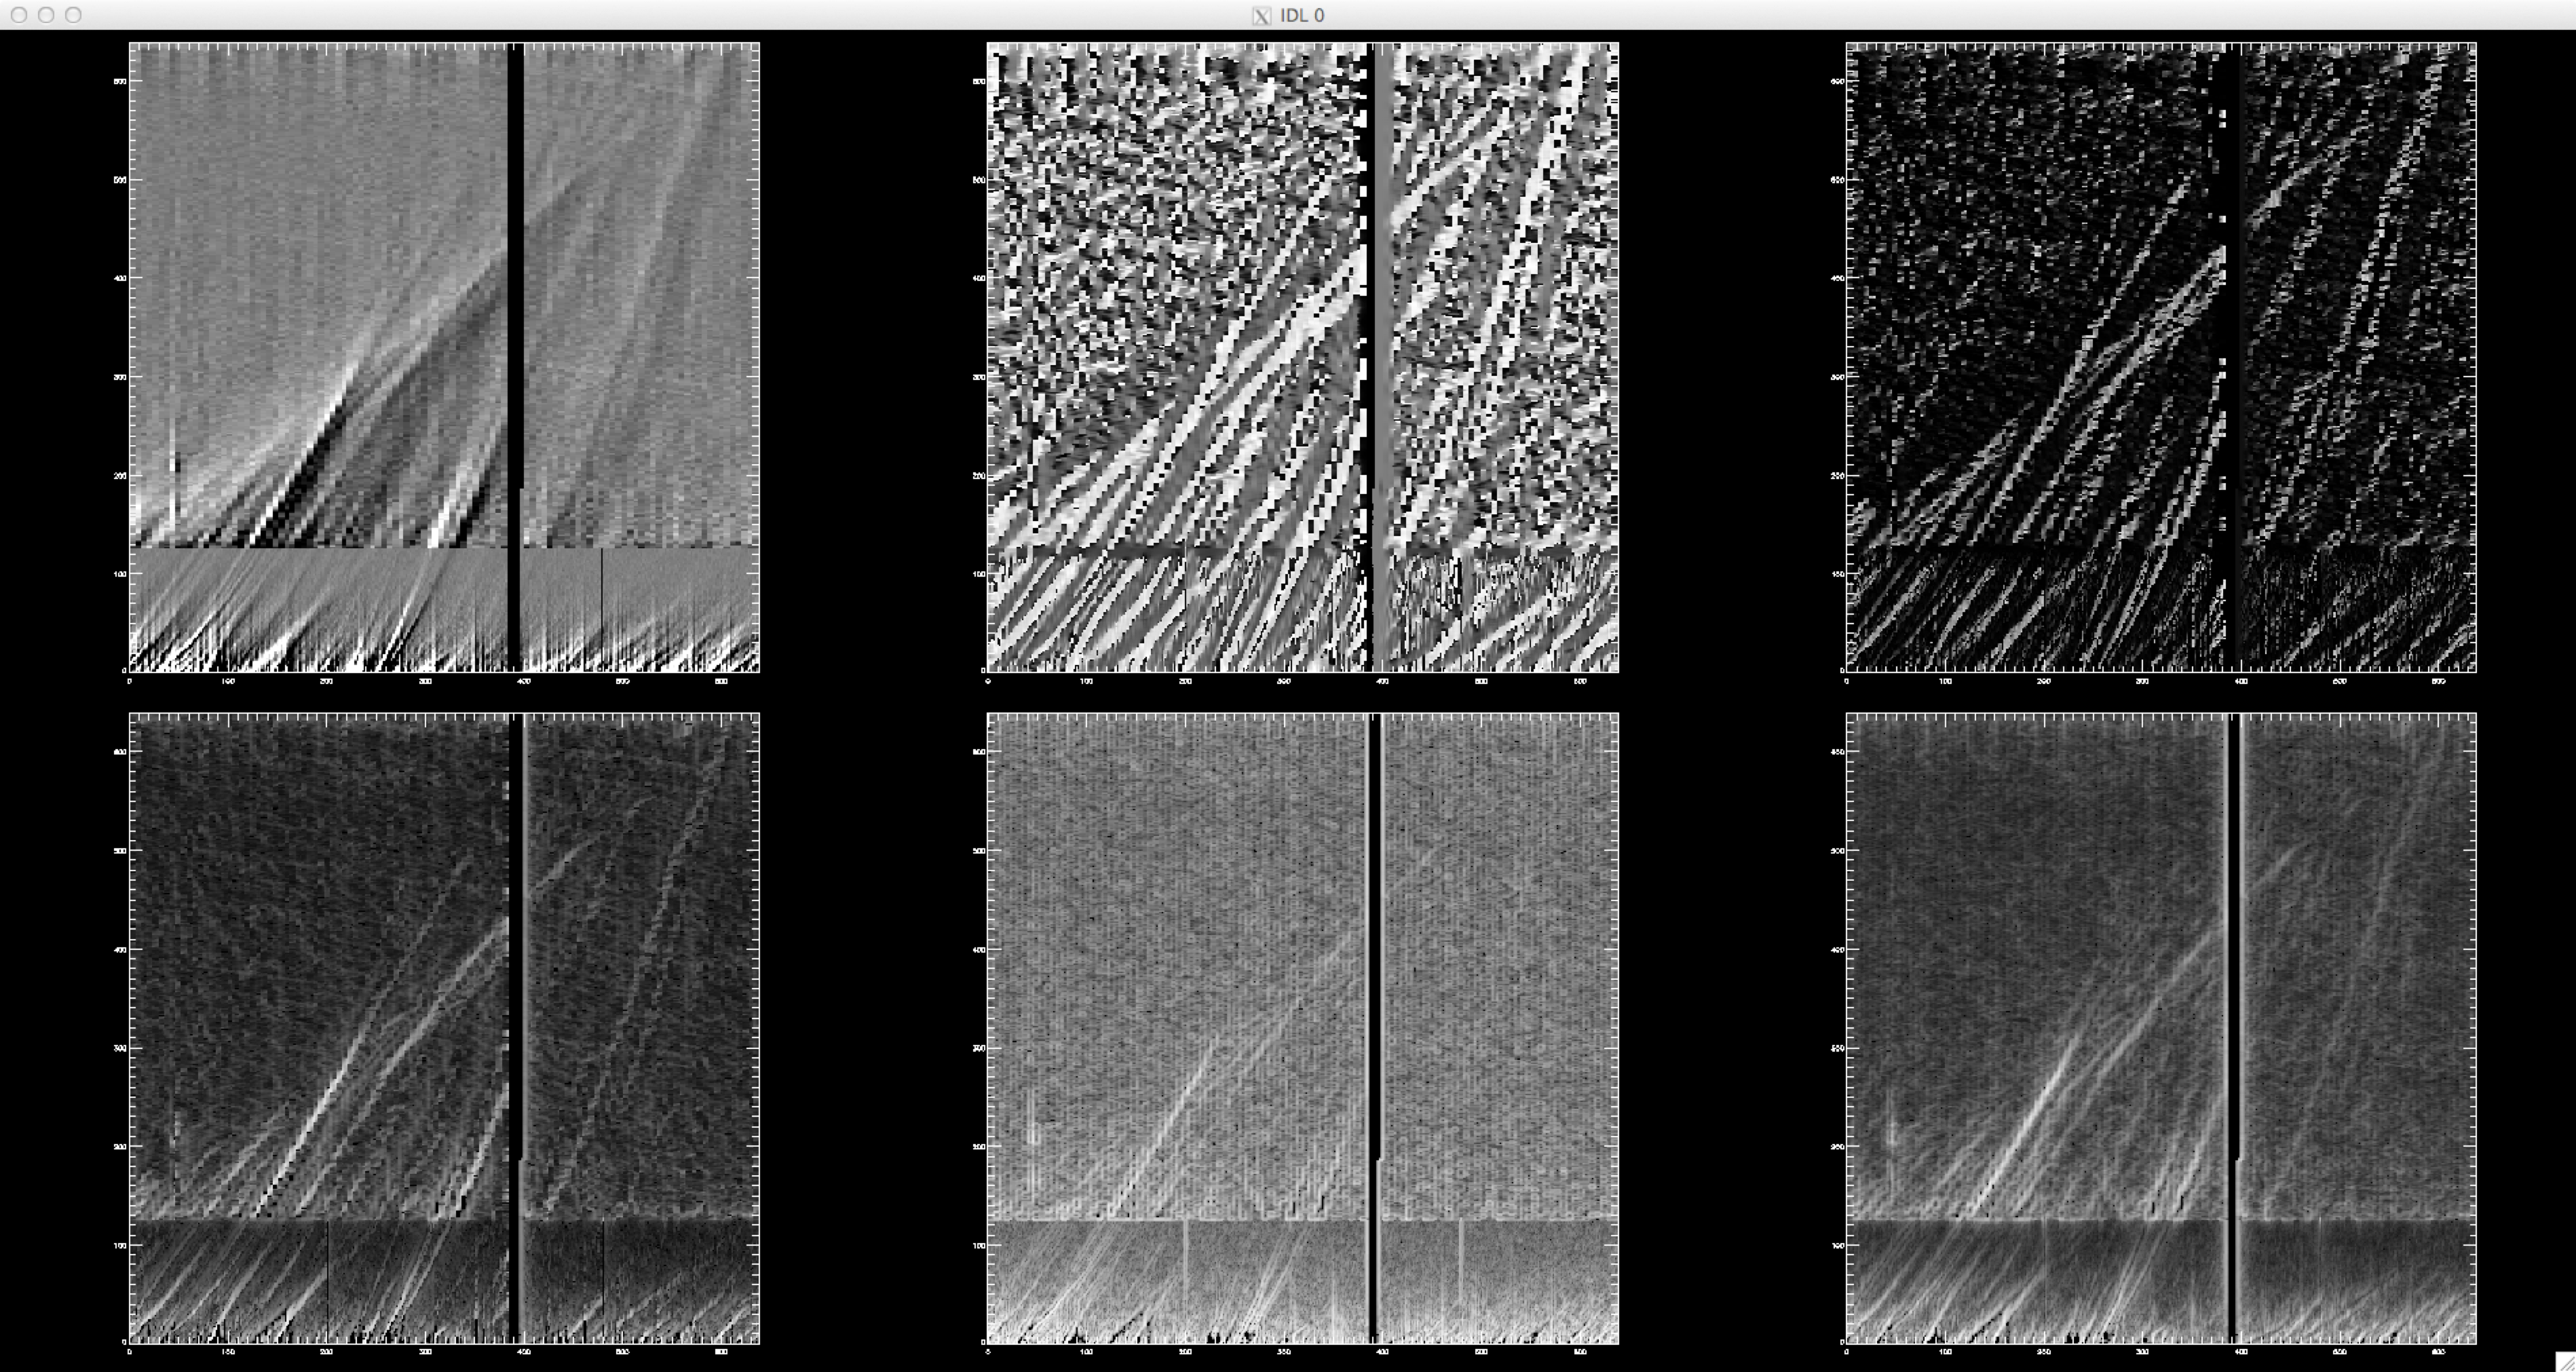
\includegraphics[width=\textwidth]{../images/comparison_all.png}
\caption{The application of a multiscale filter (namely the Canny-Atrous of Young et al. 2008) to the original HIs J-map shown in the top left image. The subsequent images combine the magnitude and angular information from the filtering process in different ways to highlight and contrast the structures.}
\label{comparison_all}
\end{figure}

\begin{figure}[]
\centering
\includegraphics[width=\textwidth]{../images/edges_thr.png}
\caption{A pixel-chaining algorithm may be applied to trace the edges revealed by the multiscale filtering, at various levels of thresholds.}
\label{edges_thr}
\end{figure}


\section{Ongoing efforts:}

It is planned to combine these aspects of work such that it be possible to cross-correlate / inspect the structures that would be characterised in both the images and the J-maps, to ensure that the most appropriate CME structures be tracked and catalogued.

With these codes in place, a subset of the data may be inspected to produce an initial deliverable in the form of the intended final exhaustive CME list and their catalogued properties.


%%%%%%%%%%%%%%%%%%



\end{document}
